% !TEX encoding = UTF-8 Unicode
\documentclass{article}

\usepackage{polski}
\usepackage[utf8]{inputenc}
\usepackage{subfig}
\usepackage{multirow}
\usepackage{graphicx}

\usepackage[a4paper, left=2.5cm, right=2.5cm, top=3.5cm, bottom=3.5cm, headsep=1.2cm]{geometry}

\linespread{1.3}
\begin{document}
	
	\begin{titlepage}
		\centering
		{\scshape\LARGE Politechnika Wrocławska \par}
		{\scshape\Large Katedra Informatyki Technicznej\par}
		
		\vspace{1cm}
		{\scshape\Large Inżynieria Oprogramowania\par}
		\vspace{1.5cm}
		{\huge\bfseries Identyfikacja klas reprezentujących logikę biznesową projektowanego oprogramowania, definicja atrybutów i 	operacji klas oraz związków między klasami - na podstawie
			analizy scenariuszy przypadków użycia. Opracowanie
			diagramów klas i pakietów. Zastosowanie projektowych
			wzorców strukturalnych i wytwórczych\par}
		\vspace{2cm}
		{\Large\itshape Magdalena Biernat\par}
		{\Large\itshape Mateusz Bortkiewicz\par}
		\vfill
		Opiekun\par
		prof. dr hab. inż. Jan Magott 
		
		\vfill
		{\large \today\par}
	\end{titlepage}
	\newpage
	
	\section{Wprowadzenie}
	Sprawozdanie dotyczy siódmych zajęć. Na tych laboratoriach kontynuowaliśmy swój projekt. 
	
	\subsection{Cel laboratorium}
Tworzenie modelu projektowego programowania opartego na
identyfikacji klas, reprezentujących logikę biznesową projektowanego systemu. Należy dokonać definicji atrybutów klas oraz związków między klasami - na podstawie analizy scenariuszy przypadków użycia.
	
	\subsection{Plan pracy}
	Zadania wykonaliśmy wg instrukcji 5:
	
	\begin{itemize}
		\item Wykonanie diagramu klas
	\end{itemize}
	\newpage
	\section{Laboratorium}
	\subsection{Wykonanie diagramu klas}
\begin{figure}[!ht]
	\centering
	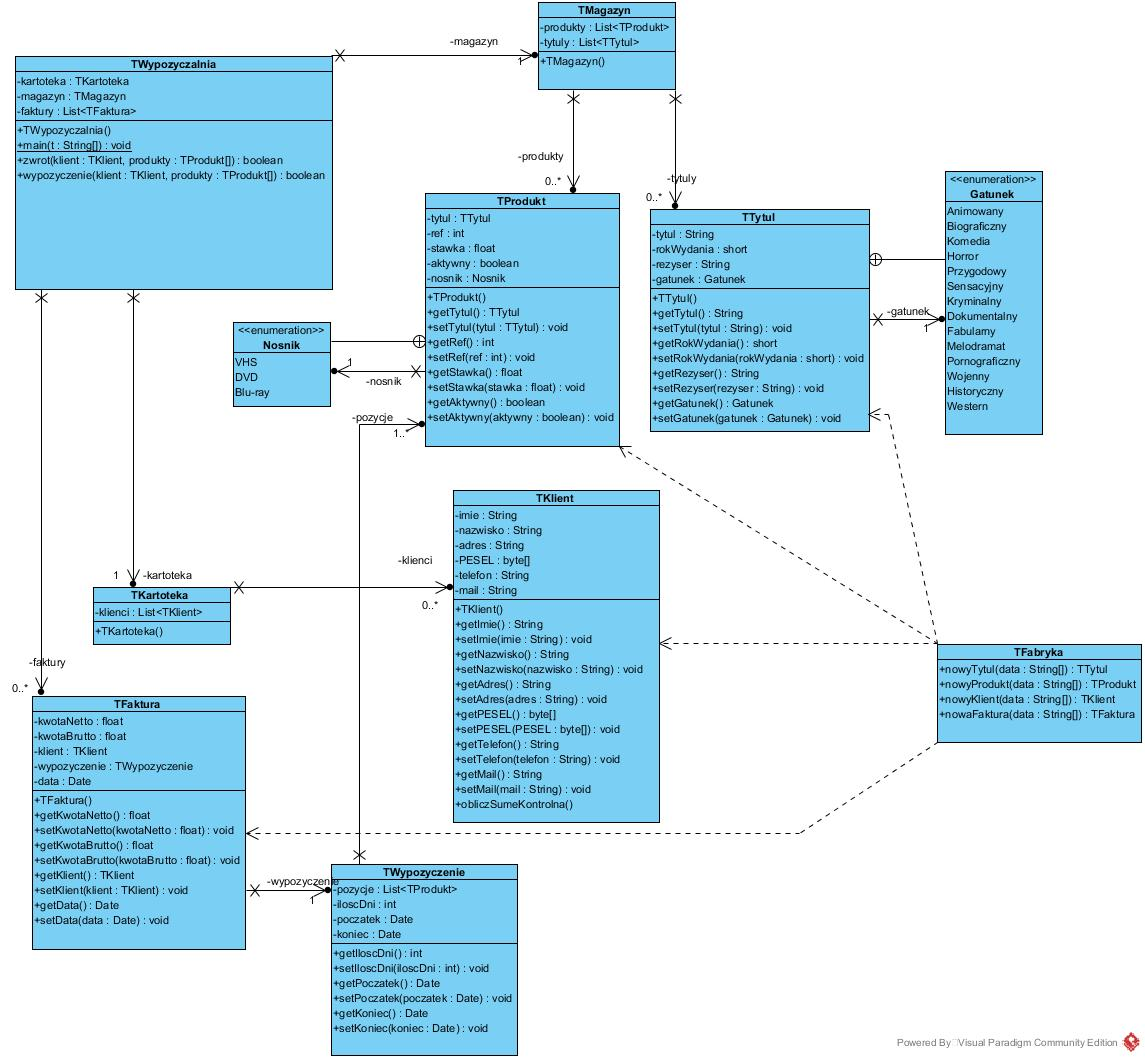
\includegraphics[width=17cm]{diagram_klas.jpg}
	\caption{Stworzony diagram klas}
	\label{fig:obrazek 1}
\end{figure}
	\newpage
	\subsection{Opracowanie diagramów}
	\subsubsection{Analiza wspójności}
	Wykryto 3 główne klasy typu „Entity” ze względu na odpowiedzialność:
	\begin{itemize}
	\item TWypozyczalnia (PU: Wypożyczenie, PU Przyęcie towaru)
	\item TWypożyczenie (PU: Obliczanie terminu zwrotu i kosztów wypożczenia)
	\item TFabrtka (PU: Wstawienei paragonu/faktury za wypożczenie)
	\end{itemize}	
TWypozyczenie
- obliczanie terminu zwrotu i kosztów wypożyczenia

TWypożyczalnia
- wypożyczenie
- przyjęcie towaru

TFabryka
- wystawienie paragonu/faktury za wypożyczenie

Nie znalazłam tego w diagramie klas
?- obliczanie przedawnienia i kosztu przetrzymania
?- wystawienie potwierdzenia za przetrzymanie
?- szukanie wypożyczenia
?- szukanie klienta
?- szukanie pozycji
\subsubsection{Analiza zmienności}
Wykryto rozszrzenie klasy TProdukt - Nosnik
Wykryto rozszrzenie klasy TTytul - Gatunek
Wykryto związki między klasami:
\begin{itemize}
	\item Klasa TMagzayn zawiere listy obiektów klas TProdukt i TTytul
	\item Klasa TKartoteka zawiera listę obiektów klasy TKlient
	\item Klasa TFabrtyka tworzy nowe obiekty klas: TTytul, TProdukt, TKlient oraz TWypozyczenie
	\item Klasa TWypozyczalnia rozpoczyna cały proces wypożyczenia i zwrotu produktu
	\item Klasa TFaktura pobiera dane z TWypozyczenie, żeby wystawić fakturę
	\item Klasa TWypozyczenie pobiera dane z TProdukt, żeby zainicjować wypożczenie produktu
	\item Klasa TKartoteka zawiera listę obiektów klasy TKlients
\end{itemize}	
\end{document}